\documentclass{article}
\usepackage{amsthm}
\usepackage[margin=1in]{geometry}
\usepackage{graphicx} 
\usepackage{booktabs}
\usepackage{placeins}
\usepackage{tabularx}
\usepackage{hyperref}
\usepackage{amssymb, amsmath}
\usepackage{algorithm}
\usepackage[noend]{algpseudocode}
\usepackage{booktabs}
\usepackage[font=small, labelfont=bf, labelsep=period]{caption}
\usepackage{cite}
\usepackage{url}

\theoremstyle{definition}
\newtheorem{prediction}{Prediction}

\newtheorem{lemma}{Lemma}[subsection]
\renewcommand{\thelemma}{\arabic{subsection}.\arabic{lemma}}

\title{Finding a Range Minimum Query: A Comparison of Optimality and Practicality}
\date{October 2026}


\begin{document}

\maketitle

\begin{abstract}
In this report, five different algorithms used to find the range minimum query of a given array are analysed and compared both theoretically and practically.  Some are practical to implement such as the linear and block solutions, while the Fischer--Heun is the most theoretically optimal, and both the sparse table and segment tree sit in-between.  Each implementation of the algorithms is benchmarked, where it shows there are cases where each of the five algorithms is the best to implement.  However, for arrays of exponentially large sizes, with many queries, the Fischer--Heun is demonstrated as the most optimal implementation.
\end{abstract}

\section{Introduction}
Finding the smallest element in some  unsorted array of integers, $A = \{a_1, a_2\dots, a_n\}$, can be done in two different ways.  The first being a linear search over the array, such that each element is compared to the smallest found value, and the minimum of those two is stored.  The second is sorting the array in ascending order and returning the first value.  In every scenario the linear search beats the sorting approach, with $\Theta(n)$ instead of $\Theta(n\log{n})$.
\\
\\
Consider finding the smallest value in a sub-array of $A[i..j]$ where $0 \le i \le j < n$. Now the linear search is the only feasible solution here, where the previous sorting approach would disrupt the indices of the array.  It follows that, if the array never changes, then multiple queries can be made in any order.  Assuming no two indices overlap, and no duplicate queries are made, then the linear search is still the best approach.  This is because you will scan at most $n$ elements.
\\
\\
Let $q$ be the set of all queries.  Now consider the alternative where multiple queries can be made such that any two can overlap and duplicates exist.  The linear solution now runs $\theta(q\cdot n)$.  The key observation is how elements are reprocessed for any overlapping ranges.
\\
\\
The goal of the range minimum query problem is to sacrifice pre-processing speed for querying speed, such that the reprocessing of elements is reduced as much as possible.  So, we provide a theoretical and analytical comparison of the known solutions to this problem: linear, block, segment tree, sparse table, and Fischer--Heun~\cite{fischer2006, cs166rmq2}.
\\
\\
Each individual algorithm is provided with an overall analysis on its complexities and requirements.  These are then compared both theoretically and practically, where real benchmarks of running time and resource consumption are provided.  Our method of experimentation is detailed, and the repository containing all the necessary code and resources can be found \href{https://github.com/replicantStarr/Range-Minimum-Query-Implementation-Comparisons}{here}.

\section{Theoretical Analysis}
\textbf{Helpful notation.} Let $A$ be an arbitrary array of integers, and $Q$ be the array of queries which will call query.
\\
\\

\subsection{Linear}
\paragraph{Algorithm.}
A simple scan over each element in $a[i..j]$.

\begin{algorithm}[H]
\caption{Linear Search}
\label{alg:linear}
\begin{algorithmic}[H]
\Function{Query}{$i, j$}
    \State $\mathit{m} \gets A[i]$
    \For{$i\prime \gets i$ \textbf{to} $j$}
        \State $\mathit{m} \gets \min(m, A[i\prime])$
    \EndFor

    \State \Return m
\EndFunction
\end{algorithmic}
\end{algorithm}

\paragraph{Running Time.}
Runs in $\Theta(j - i)$, where each element in $A[i..j]$ must be processed once.

\paragraph{Memory Consumption.}
Only a reference to the array is stored, and therefore $O(1)$.  Without a reference, then exactly $n$ 32-bit integers are stored with complexity $O(n)$.

\subsection{Block}

\paragraph{Algorithm.}
The minimum of all possible queries for $A$ is pre-processed into $m[i][j]$ for querying.

\begin{algorithm}[H]
\caption{Linear Search}
\label{alg:block}
\begin{algorithmic}[H]
\Function{Construct}{A}
    \For{$i \gets 1$ \textbf{to} len(A)}
        \For{$i \gets 1$ \textbf{to} len(A)}
            \State $M[i][j] \gets \min(M[i][j-1], A[j])$
        \EndFor
    \EndFor
\EndFunction
\\
\Function{Query}{$i, j$}
    \State \Return $M[i][j]$
\EndFunction
\end{algorithmic}
\end{algorithm}

\paragraph{Running Time.}
\textsc{Construct} runs in $\Theta(n^2)$.
\textsc{Query} runs in constant time $O(1)$.

\paragraph{Memory Consumption.}
\textsc{Construct} stores the result of exactly $n^2$ 32-bit integers.

\subsection{Segment Tree}
\paragraph{Algorithm.}
A binary tree in which each node stores the minimum of a block of $A$: leaves hold single elements, and each internal node holds the minimum of its two children. $A$ is padded with $\infty$ to the next power of two $L$ ($n \leq L < 2n$), giving $2L - 1$ nodes stored in a flat array $T$, with the children of node $k$ at $2k + 1$ and $2k + 2$. A query splits $[i, j]$ into $\Theta(\log{n})$
disjoint node blocks.

\begin{algorithm}[H]
\caption{Segment Tree}
\begin{algorithmic}[H]
\Function{Construct}{$A$}
  \State $n \gets \mathrm{len}(A)$, \quad $L \gets 1$
  \While{$L < n$}
    \State $L \gets 2L$
  \EndWhile
  \State $T[0..2L-2] \gets \infty$
  \For{$x \gets 0$ to $n - 1$}
    \State $T[L - 1 + x] \gets A[x]$
  \EndFor
  \For{$k \gets L - 2$ \textbf{down to} $0$}
    \State $T[k] \gets \min(T[2k+1],\ T[2k+2])$
  \EndFor
\EndFunction
\Function{Query}{$i, j$}
  \State \Return \Call{RangeMin}{$0,\ 0,\ L-1,\ i,\ j$}
\EndFunction
\Function{RangeMin}{$k, l, r, i, j$}
  \If{$j < l$ \textbf{or} $r < i$}
    \State \Return $\infty$ \Comment{block disjoint from $[i, j]$}
  \EndIf
  \If{$i \leq l$ \textbf{and} $r \leq j$}
    \State \Return $T[k]$ \Comment{block inside $[i, j]$}
  \EndIf
  \State $m \gets \lfloor (l + r) / 2 \rfloor$
  \State $\mathit{left} \gets \Call{RangeMin}{2k+1,\ l,\ m,\ i,\ j}$
  \State $\mathit{right} \gets \Call{RangeMin}{2k+2,\ m+1,\ r,\ i,\ j}$
  \State \Return $\min(\mathit{left},\ \mathit{right})$
\EndFunction
\end{algorithmic}
\end{algorithm}
 
\textbf{Correctness.} Every node holds the minimum of its block, since it is built from its two children. A query returns $\infty$ for a block disjoint from $[i, j]$, the stored value for a block inside $[i, j]$, and otherwise the smaller answer of the two children, whose blocks partition the
node's block. Unlike the sparse table, the pieces never overlap, so this also works for range sums.
 
\textbf{Running Time.} Construct writes each of the $2L - 1 < 4n$ nodes once, so it runs in $\Theta(n)$. Query only expands blocks that partially overlap $[i, j]$, at most two per level, so it visits at most four nodes per level and runs in $O(\log n)$. Neither depends on the values in $A$.
 
\textbf{Memory Consumption.} $T$ stores $2L - 1$ 32-bit integers: $2n - 1$ when $n$ is a power of two, and up to about $4n$ otherwise, so $\Theta(n)$. For $n = 2^{20}$ this is about $8$ MB, against $88$ MB for the sparse table.

\subsection{Sparse Table}
\textbf{Algorithm.} Builds a table $M$ where $M[x][p]$ stores $\min(A[x..x + 2^p - 1])$, the block of length $2^p$ starting at $x$. Column $0$ is the array itself, and each later column combines two adjacent blocks from the column before it. A query is the minimum of two overlapping lookups. $\lfloor \log_2 \ell \rfloor$ is precomputed for every length $\ell \leq n$, so Query reads $p$ from a table.
 
\begin{algorithm}[H]
\caption{Sparse Table}
\begin{algorithmic}[H]
\Function{Construct}{$A$}
  \State $n \gets \mathrm{len}(A)$
  \For{$x \gets 0$ to $n - 1$}
    \State $M[x][0] \gets A[x]$
  \EndFor
  \For{$p \gets 1$ to $\lfloor \log_2 n \rfloor$}
    \For{$x \gets 0$ to $n - 2^p$}
      \State $M[x][p] \gets \min(M[x][p-1],\ M[x + 2^{p-1}][p-1])$
    \EndFor
  \EndFor
\EndFunction
\Function{Query}{$i, j$}
  \State $p \gets \lfloor \log_2(j - i + 1) \rfloor$
  \State \Return $\min(M[i][p],\ M[j - 2^p + 1][p])$
\EndFunction
\end{algorithmic}
\end{algorithm}
 
\textbf{Correctness.} For a query of length $m = j - i + 1$, $p = \lfloor \log_2 m \rfloor$ gives
$2^p \leq m < 2^{p+1}$. Each block fits inside $A[i..j]$, and together they cover it, possibly
overlapping. The overlap is harmless because $\min(v, v) = v$, but a smaller $p$ would leave a
gap. The same trick fails for range sums, where the overlap would be counted twice.
 
\textbf{Running Time.} Each of the $\lfloor \log_2 n \rfloor$ columns after column $0$ fills at most $n$ entries,
and all but the last fill more than $n/2$, so Construct runs in $\Theta(n \log n)$. Query does two
table reads and one comparison, so it runs in $O(1)$. Neither depends on the values in $A$, only
on $n$.
 
\textbf{Memory Consumption.} Construct stores $n \times (\lfloor \log_2 n \rfloor + 1)$ 32-bit
integers, giving $\Theta(n \log n)$. For $n = 2^{20}$ this is about $88$ MB, against $4$ MB for
the array itself.

\subsection{Fischer--Heun}
\paragraph{Algorithm.}
Divides $A$ into blocks of size $b$.  Blocks of different values can have the same index of minimum value (refer).  A block has its own table, which is then stored under a hashed Cartesian number.  Then for all other blocks, if the Cartesian number has already been processed, it will skip creating the same table.  The minimum value of each block is stored in a summary array, and a sparse table is constructed around the summary array, such that a query will take most of its values here instead of Cartesian table.  This is the most theoretically optimal algorithm.

\begin{algorithm}[H]
\caption{Fischer--Heun}
\label{alg:Fischer--Heun}
\begin{algorithmic}[1]
\Function{Construct}{$A$}
    \State $b \gets \lfloor \frac{1}{2} \lfloor \log_2 n \rfloor \rfloor$
    \If{$b < 2$} \Return \Comment{Queries use a linear scan}
    \EndIf
    \ForAll{blocks $B_k$ of $A$}
        \State $(c, m) \gets$ \Call{CartesianNumber}{$B_k$}
        \If{$c \notin H$}
            \State $H[c] \gets |\mathit{Tables}|$
            \State Append \Call{BuildTable}{$B_k$} to $\mathit{Tables}$
        \EndIf
        \State $R[k] \gets H[c]$
        \State $S[k] \gets m$
    \EndFor
    \State Build a sparse table over $S$
\EndFunction
\Statex
\Function{CartesianNumber}{$B$}
    \State $c \gets 0$; $m \gets B[0]$; $\mathit{stack} \gets \emptyset$
    \ForAll{$x$ in $B$}
        \State $m \gets \min(m, x)$
        \While{$\mathit{stack} \neq \emptyset$ \textbf{and} $\mathit{top}(\mathit{stack}) > x$}
            \State Pop $\mathit{stack}$; $c \gets 2c$
        \EndWhile
        \State Push $x$; $c \gets 2c + 1$
    \EndFor
    \State \Return $(c, m)$
\EndFunction
\Statex
\Function{BuildTable}{$B$}
    \For{$i \gets 0$ \textbf{to} $|B| - 1$}
        \State $T[i][i] \gets i$
        \For{$j \gets i + 1$ \textbf{to} $|B| - 1$}
            \If{$B[j] < B[T[i][j - 1]]$}
                \State $T[i][j] \gets j$
            \Else
                \State $T[i][j] \gets T[i][j - 1]$
            \EndIf
        \EndFor
    \EndFor
    \State \Return $T$
\EndFunction
\Statex
\Function{Query}{$l, r$}
    \If{$b < 2$} \Return minimum of $A[l..r]$ by linear scan
    \EndIf
    \State $s \gets \lfloor l / b \rfloor$; $e \gets \lfloor r / b \rfloor$
    \State $T_s \gets \mathit{Tables}[R[s]]$; $T_e \gets \mathit{Tables}[R[e]]$
    \If{$s = e$}
        \State \Return $A[sb + T_s[l - sb][r - sb]]$
    \EndIf
    \State $v \gets \min(A[sb + T_s[l - sb][b - 1]],\; A[eb + T_e[0][r - eb]])$
    \If{$s + 1 < e$}
        \State $v \gets \min(v, \textsc{SparseQuery}(s + 1, e - 1))$
    \EndIf
    \State \Return $v$
\EndFunction
\end{algorithmic}
\end{algorithm}

\paragraph{Running Time.}
\textsc{Construct} computes a Cartesian number for each block in $O(b)$ using a stack, which is $O(n)$ across all blocks, and each hash map lookup takes expected $O(1)$. Each distinct shape adds a table in $O(b^2)$. The sparse table covers about $n/b$ block minimums and therefore takes $O(\frac{n}{b} \log \frac{n}{b})$, which is $O(n)$ since $b = \Theta(\log n)$. \textsc{Query} performs two table lookups and one sparse table query, each of which takes constant time, so it runs in $O(1)$.

\paragraph{Memory Consumption.}
The summary and block references each store about $n/b$ 32-bit integers, and the sparse table stores about $\frac{n}{b} \log \frac{n}{b}$, which is $O(n)$. Each distinct shape adds a table of $b^2$ integers. The input array is kept by reference, so it is not counted, although it must remain available for queries. Measured memory stayed between about 16 and 20 bytes per element from $n = 2^{10}$ to $n = 2^{24}$ on random input (Figure~\ref{fig:b1}).

\paragraph{Cartesian Numbers.}
A block's Cartesian tree can be built with a stack, and the sequence of pushes and pops describes its shape. Each push is recorded as a 1 and each pop as a 0, which gives a binary number of at most $2b$ bits. Blocks with the same number have the same shape, so they share a table. A 32-bit integer can therefore represent any block size up to $b = 16$. Ascending input needs very few tables, while random input needs many, which explains the difference shown in Figure~\ref{fig:c1}.

\paragraph{Optimal Block Size.}
Smaller blocks produce a larger sparse table, while larger blocks produce more distinct shapes with larger tables. The standard analysis uses $b = \frac{1}{4} \log_2 n$~\cite{cs166rmq2}, which limits the possible shapes to about $4^b = \sqrt{n}$, so all tables together take $o(n)$ space~\cite{bender2000, fischer2006}. This implementation uses $b = \frac{1}{2} \log_2 n$, which suffices for the as part of the bound of minimal values to allow $n$ to dominate. However, the number of tables can never exceed the number of blocks, and memory remained flat on the inputs tested. At $n = 2^{20}$, build time and memory are lowest at $b = 9$, close to the default of $b = 10$ (Figure~\ref{fig:f1}). Query time was not measured at each block size, so this result covers build cost only.

\section{Theoretical Comparison}
\subsection{Running Time}
\subsubsection{Construction}
Between all five algorithms, the theoretically best construction is naive linear with $O(1)$.  Then, the second best is the segment tree $O(n)$, where each of the nodes are constructed as children, and step up each time until the root such that the minimum value at that point is stored.  Fischer--Heun is also $O(n)$, however in scenarios where the $A$ contains a unique Cartesian number per block, the construction can require more operations.  Sparse table is complete in $O(n\cdot \log(n))$, and requires far more operations than the Fischer--Heun.  Out of all, the most inefficient is block $O(n^2)$, where each possible query is saved along with its answer.

\subsubsection{Memory Consumption}
The linear solution only takes a reference to $A$, therefore being the most optimal for memory consumption.  For powers of 2, the segment tree will store exactly $2n - 1$ nodes, which is far less than the sparse table $n\cdot \log_2(n)$.  Additionally, Fischer--Heun can store far less than sparse table where $A$ has several similar blocks.  At worst, it will contain $\frac{n}{b}$ tables of $b\times b$, along with its summary array and sparse table.  Out of all, the least memory efficient is block, with $n\times n$ 32-bit integers stored.

\subsubsection{Querying}
As discussed earlier, linear is $\Theta(n)$ for queries.  The block algorithm is a constant time query and is equally fastest querying.  Using a sparse table is effectively the same, with the exception of needing to compare two smaller values making it an extra step. Fischer--Heun is next, with also a constant time query, for larger queries it must use the summary sparse table.  Querying with a segment tree is complete in $O(\log(n))$, therefore making it the least optimal outside of linear for larger values.

\subsubsection{Best Choice}
Theoretically, Fischer--Heun is the best choice with $O(n)$ construction, and $O(1)$ querying.  However as demonstrated in later sections, time complexity should not be the only consideration when solving problems.

\section{Predictions}

\begin{prediction}\label{pred:worst}
The linear solution will be the fastest construction for all $0 \le len(a) \le 2^{24}$
\end{prediction}
\begin{proof}[Reason]
Construction should be simply storing the reference of the provided array in memory.  This is a constant time operation and the only constant time construction.
\end{proof}


\begin{prediction}\label{pred:avg}
The linear construction will consume the least amount of memory for all $0 \le len(a) \le 2^{24}$.
\end{prediction}
\begin{proof}[Reason]
The absolute lower bound for memory consumption is $\Omega(n)$, as a query can be $a[i..i]$ and so every value must be stored regardless of implementation.  The linear search is the only one which stores the exact array only once.
\end{proof}

\begin{prediction}\label{pred:best}
Linear will have the overall slowest querying for all $0 \le len(a) \le 2^{24}$.
\end{prediction}
\begin{proof}[Reason]
For smaller sizes of $0 \le n \le 2^3$, the linear search will be the fastest.  However, as $n$ approaches $2^{14}$ it will become a near exponential outlier.
\end{proof}

\begin{prediction}\label{pred:best}
The block solution will have the overall slowest construction for $2^3 \le n \le 2^{24}$.
\end{prediction}
\begin{proof}[Reason]
The block represents the opposite of linear, and stores the absolute maximum possible queries in $a$, $\frac{n(n+1)}{2}$.  It's reasonable to believe that whilst the earlier values of $n$ will be cheap, it will consume the most amount of memory exponentially compared to others.
\end{proof}

\begin{prediction}\label{pred:best}
It follows, block solution will have the fastest querying for all $0 \le n \le 2^{24}$.
\end{prediction}
\begin{proof}[Reason]
If every possible query is stored in some $m[i][j]$, then the retrieval is a constant time.  It is practically impossible to beat this.
\end{proof}

\begin{prediction}\label{pred:best}
The Fischer--Heun and Sparse Table will be the most similar in memory consumption for all $0 \le n \le 2^{24}$.
\end{prediction}
\begin{proof}[Reason]
Fischer--Heun is just contains a sparse table per block, instead of the entirety of $a$.  Whilst Fischer--Heun will also store a reference to $a$ and a summary array, the storing of the sparse table will dominate all else.
\end{proof}

\begin{prediction}\label{pred:best}
The sparse table will be faster than the segment tree for querying
\end{prediction}
\begin{proof}[Reason]
Fischer--Heun is just contains a sparse table per block, instead of the entirety of $a$.  Whilst Fischer--Heun will also store a reference to $a$ and a summary array, the storing of the sparse table will dominate all else.
\end{proof}

\begin{prediction}\label{pred:best}
For block sizes $2 \le b \le 2^4$, construction will take longer where $b$ is far out of proportion with $\frac{1}{2}\log_2{n}$.   
\end{prediction}
\begin{proof}[Reason]
The complexity changes with the block size, and therefore the construction will take longer for the same $a$.
\end{proof}

\begin{prediction}\label{pred:best}
Fischer--Heun construction will take the longest aside from block, despite the running time $O(n)$.
\end{prediction}
\begin{proof}[Reason]
A better time complexity does not always mean a faster result.  This can be determined by how many factors you choose to associate $n$ with inside the implementation.  Fischer--Heun exists to precisely do that, where the $n$ will beat constructing sparse tables for each block.
\end{proof}

\begin{prediction}\label{pred:best}
Segment tree will be the slowest query of the non-naive solutions for all $1 \le n \le 2^{24}$.
\end{prediction}
\begin{proof}[Reason]
Outside of linear, all solutions query in constant time.  Segment tree does not, and therefore there is no reason to believe this.
\end{proof}

\begin{prediction}\label{pred:best}
Although all being constant, there will be a noticeable difference between block, sparse table and Fischer--Heun querying for all $2^3 \le n \le 2^{24}$.
\end{prediction}
\begin{proof}[Reason]
The sparse table and Fischer--Heun take extra steps despite being constant time query.  I believe these extra steps will be shown in nanoseconds.
\end{proof}

\section{Experimental Methodology}
\subsection{Benchmark Source}
The benchmarks are all written as C++ source code with the Google Benchmark library.  These can be compiled and run locally, there are four types.

\begin{table}[H]
    \centering
    \small
    \caption{Benchmark suite, giving 429 parameter combinations per run. Main sizes are $n = 2^{4}$ to $2^{24}$ in steps of a factor of 4, with Naive block limited to $n = 2^{14}$. Padding sizes are $n = 2^{k}$, $2^{k} + 1$ and $1.5 \times 2^{k}$ for even $k$ from 10 to 22.}
    \label{tab:benchmarks}
    \resizebox{\textwidth}{!}{%
    \begin{tabular}{lllll}
        \toprule
        \textbf{Benchmark} & \textbf{Structures} & \textbf{Input variants} & \textbf{Parameters} & \textbf{Combinations} \\
        \midrule
        Construct & All five & Random or ascending array & 11 sizes & 100 \\
        Construct, padding & Segment tree & Random array & 21 padding sizes & 21 \\
        Query & All five & Random, short, long or single-element ranges & 11 sizes & 200 \\
        Query, padding & Segment tree & Random ranges & 21 padding sizes & 21 \\
        Multiple queries & All five & Random ranges & $n \in \{2^{10}, 2^{14}, 2^{18}, 2^{22}\}$, $q \in \{1, 10^{2}, 10^{4}, 10^{6}\}$ & 72 \\
        Block size & Fischer--Heun & Random array, $n = 2^{20}$ & $b = 2$ to $16$ & 15 \\
        \midrule
        \textbf{Total} & & & & \textbf{429} \\
        \bottomrule
    \end{tabular}}
\end{table}
\subsection{Accuracy}
Benchmarking on a single machine can never truly be accurate, there is always noise and other possible disruptions.  Google Benchmark is one of the most reputable libraries when it comes to this in C++, where it will continuously complete benchmarks until it can find a stable result.  It's worth mentioning, each of the benchmarks choose to not optimise their code, so that every run can show a trend as it grows.
\\
\\
There were a total of five different repeated runs of every single benchmark, with various randomised and ascending arrays, as well as queries.  The main concern is that all randomised data was seeded, however this assists with detecting whether expected values have shifted greatly between trials.  The entire benchmarking processes was run on a single pinned core using \textit{taskset}, so that the scheduler does not interfere.  Compiler flags include \textit{-03} for code optimisation, \textit{DNDEBUG} to stop any debug checks disrupting the timing, and \textit{-march=native} to allow the use of every single possible CPU instruction.
\\
\\
The use of \textit{mallinfo2} is exclusively for glibc, and so only a linux machine would run the additional benchmarks.  It only keeps track of heap memory, so copying the input array reference would not be considered.  It places no effect on any of the timings, and simply calculates the sum of \textit{uordblks} as the small memory allocations, with \textit{hblkhd} for large allocations (these are real field names).
\\
\\
\textbf{Worth considering.}  This benchmark was only complete on a single machine with rather outdated hardware.  Whilst the overall trends in the algorithm are demonstrated, it's best to receive a wide enough sample.

\subsection{Computer Specifications}
\begin{table}[H]
    \centering
    \caption{Hardware and software configuration of the test machine.}
    \label{tab:hardware}
    \begin{tabular}{ll}
        \toprule
        \textbf{Component} & \textbf{Specification} \\
        \midrule
        CPU               & Intel Core i7-9700, 3.0\,GHz base, 4.7\,GHz maximum \\
        Cores             & 8 cores, 8 threads, no hyper-threading \\
        L1 data cache     & 32\,KiB per core \\
        L2 cache          & 256\,KiB per core \\
        L3 cache          & 12\,MiB shared \\
        RAM               & 23\,GiB \\
        \midrule
        Compiler          & GCC 16.2.1 \\
        C library         & glibc 2.43 \\
        Build tool        & CMake 4.3.0 \\
        Benchmark library & Google Benchmark v1.10.0 \\
        Compiler flags    & \texttt{-std=c++23 -O3 -DNDEBUG -march=native} \\
        \bottomrule
    \end{tabular}
\end{table}

\section{Benchmark Analysis}
\begin{table}[H]
    \centering
    \small
    \caption{}
    \label{tab:theory}
    \resizebox{\textwidth}{!}{%
    \begin{tabular}{lcccrrr}
        \toprule
        \textbf{Structure} & \textbf{Build} & \textbf{Query} & \textbf{Space} & \textbf{Build time} & \textbf{Query time} & \textbf{Bytes per element} \\
        \midrule
        Naive linear & $O(1)$ & $O(n)$ & $O(1)$ & 1.09 ns & 20 $\mu$s & 0 \\
        Naive block & $O(n^2)$ & $O(1)$ & $O(n^2)$ & not run & not run & not run \\
        Segment tree & $O(n)$ & $O(\log n)$ & $O(n)$ & 1.2 ms & 277 ns & 8 \\
        Sparse table & $O(n \log n)$ & $O(1)$ & $O(n \log n)$ & 273 ms & 44.9 ns & 128 \\
        Fischer--Heun & $O(n)$ & $O(1)$ & $O(n)$ & 22.2 ms & 74.9 ns & 16.6 \\
        \bottomrule
    \end{tabular}}
\end{table}

Table~\ref{tab:theory} compares each structure's theoretical complexity with its measured performance at $n = 2^{20}$. The results broadly follow theory, with the sparse table's build taking about 12 times longer than Fischer--Heun's and about 228 times longer than the segment tree's. However, complexity alone does not decide the ranking. Both the sparse table and Fischer--Heun have $O(1)$ queries, yet the sparse table is about 1.7 times faster. Naive linear's 1.09\,ns build reflects only the benchmark loop, as it performs no real work. All other figures in this section should be read alongside this comparison, as behaviour changes significantly with array size.

\begin{table}[H]
    \centering
    \small
    \caption{Median build time}
    \label{tab:sizes}
    \begin{tabular}{lrrrr}
        \toprule
        \textbf{Structure} & \textbf{n = $2^{12}$} & \textbf{n = $2^{14}$} & \textbf{n = $2^{20}$} & \textbf{n = $2^{24}$} \\
        Naive linear & 1.09 ns & 1.09 ns & 1.09 ns & 1.09 ns \\
        Naive block & 23.8 ms & 395 ms & not run & not run \\
        Segment tree & 3.42 $\mu$s & 14.4 $\mu$s & 1.2 ms & 59.6 ms \\
        Sparse table & 200 $\mu$s & 952 $\mu$s & 273 ms & 6.06 s \\
        Fischer--Heun & 75.9 $\mu$s & 289 $\mu$s & 22.2 ms & 679 ms \\
    \end{tabular}
\end{table}

\begin{figure}[H]
  \centering
  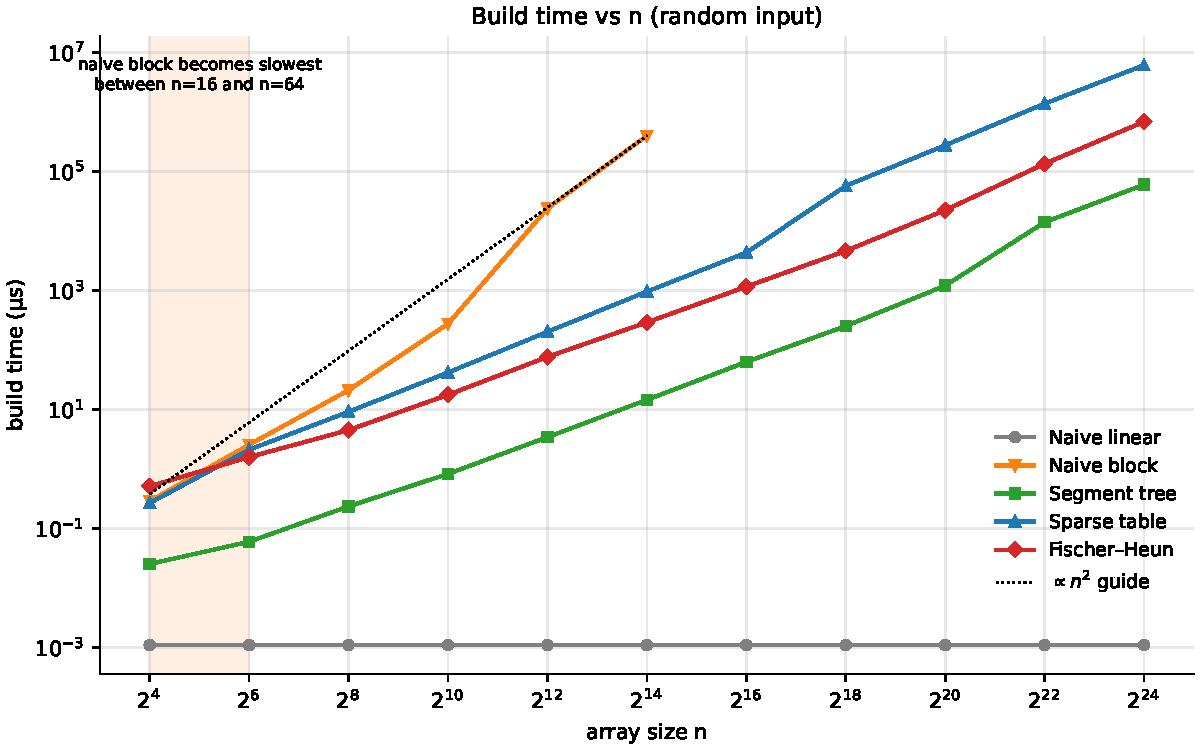
\includegraphics[width=0.8\linewidth]{figures/A1_build_time.pdf}
  \caption[Build time vs array size]{%
    \textbf{Build time vs.\ array size.}
    The build time for randomised input represented in microseconds ($\mu$s).  Array size $2^4 \le n \le 2^{24}$.}
  \label{fig:a1}
\end{figure}
Figure~\ref{fig:a1} naive linear is proven to be the fastest building at constant time, simply because it just copies the memory address of the input array.  The other algorithms represent growth with the input size, where the segment tree is the next fastest.  This is because segment tree makes $n$ leaf nodes, and then steps each level going from $n$ to $\frac{n}{2}$, $\frac{n}{4}$ until the root.  Fischer--Heun instead needs to create a summary array by finding the minimum value, then build a Cartesian number for each block, then a table and finally the sparse table.  These operations add up heavily.  The sparse table takes even longer because it builds far more entries in its own sparse table than Fischer--Heun's summary.  Naive block grows quadratically and has the longest build from $n = 2^6$.

\begin{figure}[H]
  \centering
  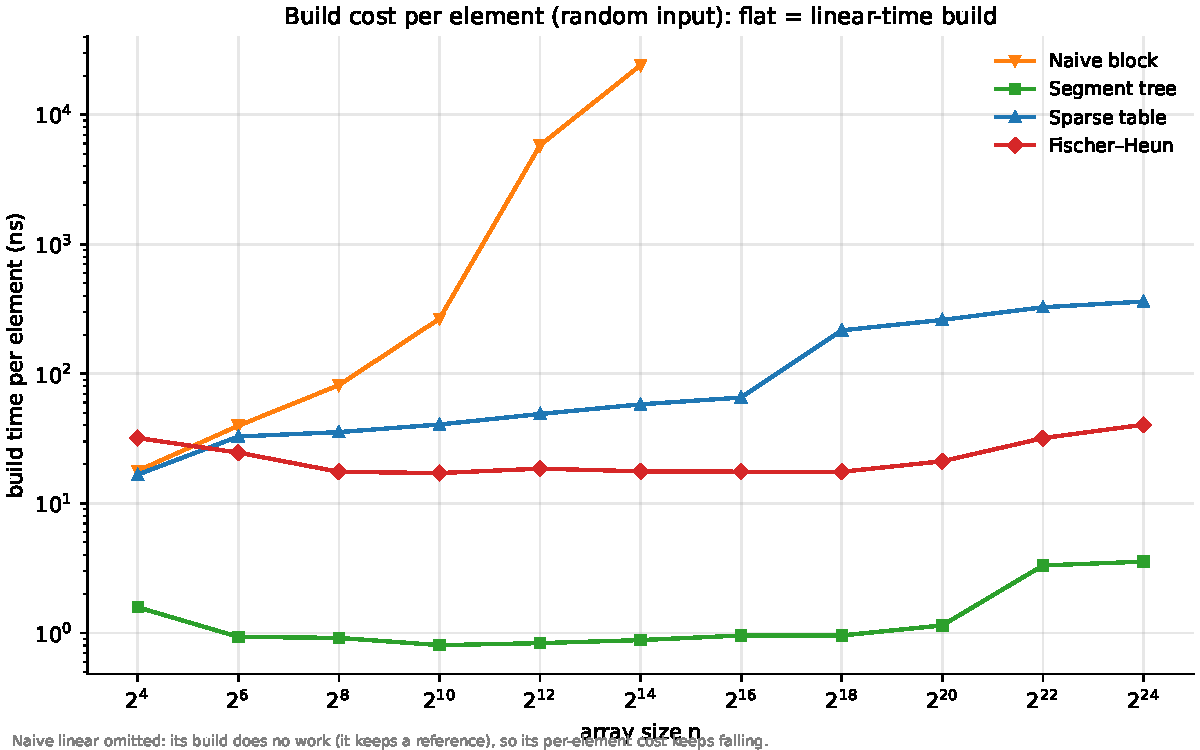
\includegraphics[width=0.8\linewidth]{figures/A2_build_per_element.pdf}
  \caption[Build time per element vs.\ array size]{%
    \textbf{Build time per element vs.\ array size.}
    Median build time / n to show build time per element.}
  \label{fig:a2}
\end{figure}
Figure~\ref{fig:a2}
Dividing build time by $n$ in Figure~\ref{fig:a2} shows how far each build departs from linear growth. The segment tree stays below 1\,ns per element from $n = 2^{6}$ to $n = 2^{18}$, and Fischer--Heun stays at about 18\,ns from $n = 2^{8}$ to $n = 2^{18}$, which is consistent with linear construction. The sparse table's cost rises by a factor of 3.9 from $n = 2^{4}$ to $n = 2^{16}$, closely matching the factor of 4 predicted by $\log n$. Above about 8\,MiB, each structure's cost rises beyond its theoretical growth. Tests with forced memory reuse show that requesting new memory from the operating system causes part of this, and for Naive block most of it. Cache effects may account for some of the remainder, though these were not measured directly.

\begin{table}[H]
    \centering
    \small
    \caption{Median build time, query time and memory on random input at selected array sizes.}
    \label{tab:sizes}
    \begin{tabular}{lrrrr}
        \toprule
        \textbf{Structure} & \textbf{n = $2^{12}$} & \textbf{n = $2^{14}$} & \textbf{n = $2^{20}$} & \textbf{n = $2^{24}$} \\
        \midrule
        \multicolumn{5}{l}{\textit{Query time (random ranges)}} \\
        Naive linear & 59.6 ns & 183 ns & 20 $\mu$s & 1.2 ms \\
        Naive block & 5.65 ns & 9.44 ns & not run & not run \\
        Segment tree & 135 ns & 160 ns & 277 ns & 501 ns \\
        Sparse table & 4.85 ns & 6.99 ns & 44.9 ns & 58.1 ns \\
        Fischer--Heun & 14.9 ns & 18.9 ns & 74.9 ns & 163 ns \\
        \bottomrule
    \end{tabular}
\end{table}

Comparing

\begin{figure}[H]
  \centering
  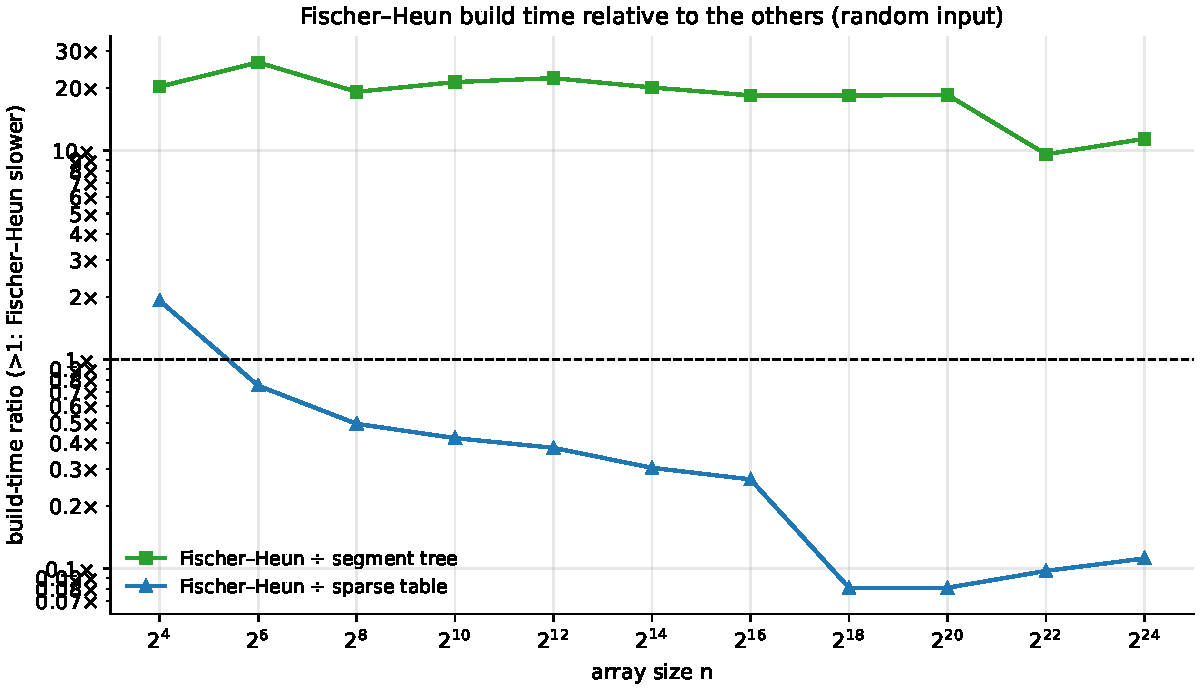
\includegraphics[width=0.8\linewidth]{figures/A3_build_ratios.pdf}
  \caption[Built ratio]{%
    Fischer--Heun is up to about 26 times slower than the segment tree, and 12 times faster than the sparse table.}
  \label{fig:a3}
\end{figure}
\textbf{Segment tree.} Figure~\ref{fig:a3} shows that Fischer--Heun's build time remains about 20 times that of the segment tree up to $n = 2^{20}$, as both grow linearly and differ by a constant factor. The ratio then halves at $n = 2^{22}$, not because Fischer--Heun improves, but because the segment tree slows. Its allocation exceeds glibc's 32\,MiB reuse limit at this size, so each build must request fresh memory from the operating system.

\textbf{Sparse table.} The ratio falls as Fischer--Heun pulls ahead with increasing size. The sparse table is faster only at $n = 2^{4}$, where it fills 54 entries, while Fischer--Heun must build 8 blocks of two values, up to two $2 \times 2$ tables, and a summary sparse table. Fischer--Heun is already faster by $n = 2^{6}$, and its ratio then falls in line with the $\log n$ factor separating their build complexities. The sharp decline at $n = 2^{18}$ is consistent with the sparse table exceeding the L3 cache while Fischer--Heun still fits. The gap then narrows slightly as Fischer--Heun also exceeds it.

\begin{figure}[H]
  \centering
  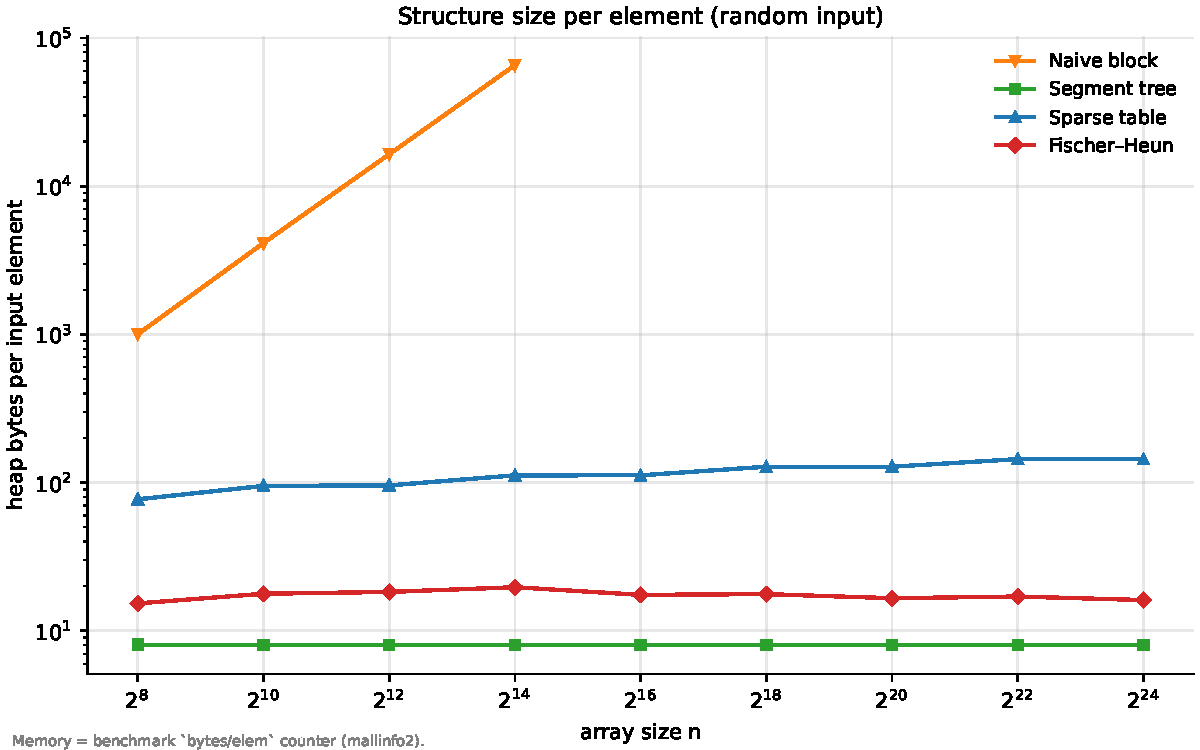
\includegraphics[width=0.8\linewidth]{figures/B1_memory.pdf}
  \caption[Structure size per element]{%
    The segment tree and Fischer--Heun are near-constant, whilst sparse table shows little growth and block shows grows proportional to n.  These are all 32-bit integers.}
  \label{fig:b1}
\end{figure}
Figure~\ref{fig:b1} shows that memory use matches each structure's theoretical growth. Naive block stores an $n \times n$ matrix of 32-bit integers, so its memory per element grows in proportion to $n$. The segment tree has the lowest memory use and stays flat at 8 bytes per element, as it is linear. These sizes are all powers of 2, which is its best case, and Figure~\ref{fig:b2} addresses other sizes. Fischer--Heun also stays nearly flat, but uses about twice the memory of the segment tree, mostly in its sparse table over blocks and its shared shape tables. The sparse table grows slowly and uses 16 to 18 times the memory of the segment tree at large sizes, as it stores a row of entries for every element.


\begin{figure}[H]
  \centering
  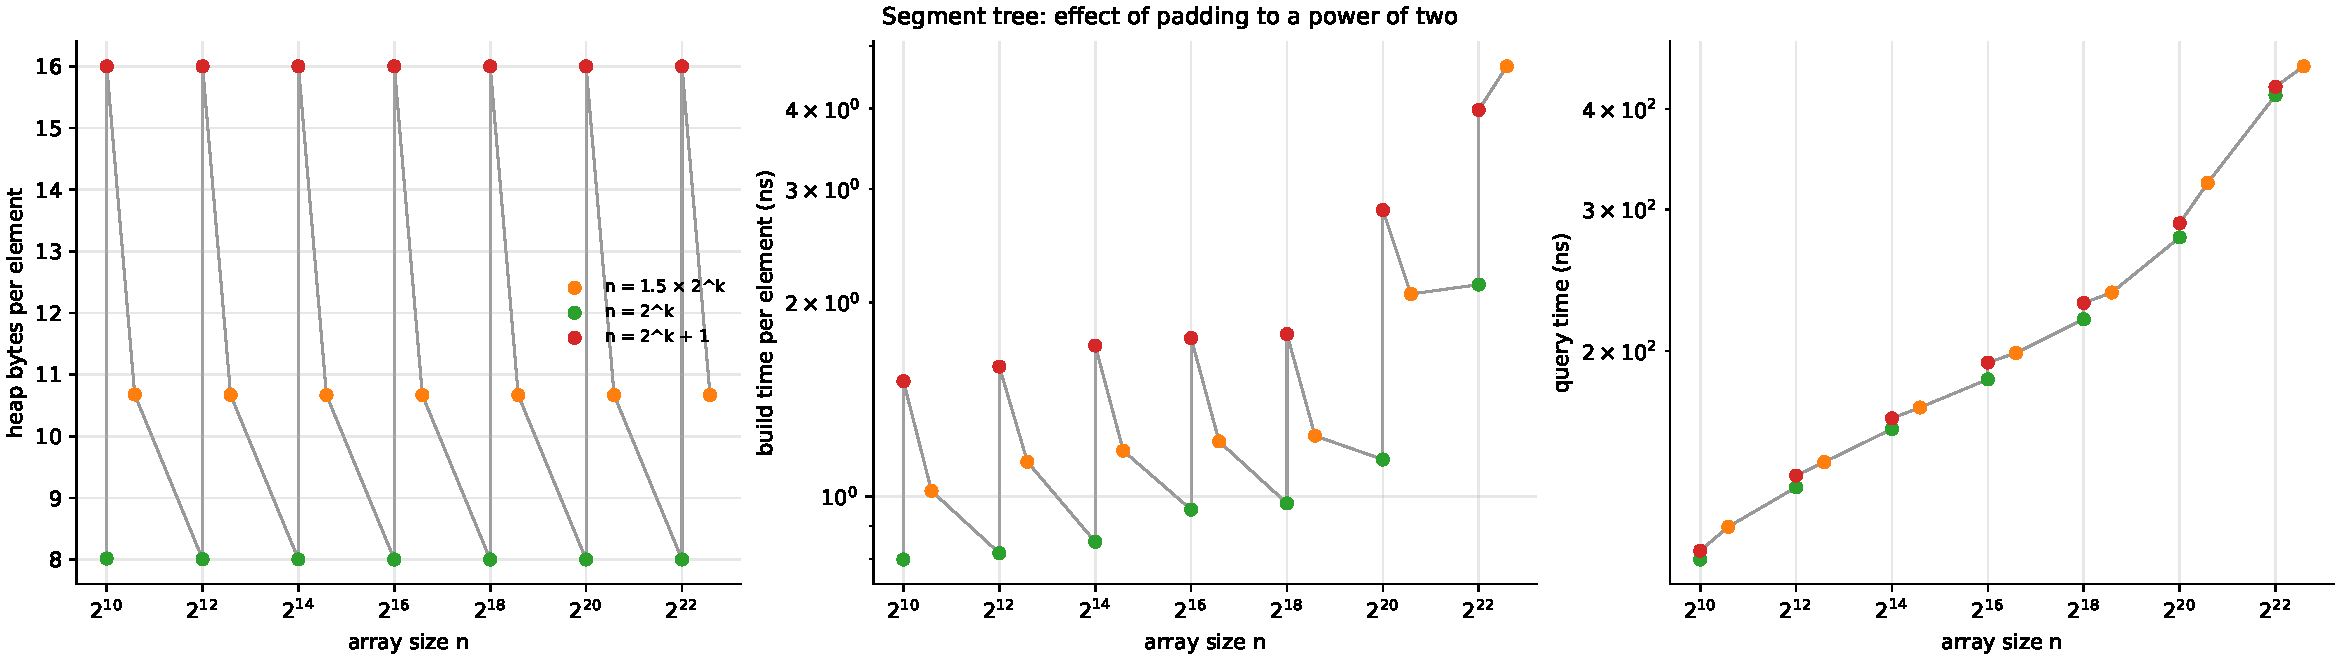
\includegraphics[width=0.8\linewidth]{figures/B2_segment_tree_padding.pdf}
  \caption[Segment Tree]{%
    Where the input size is one above a power of 2, memory doubles per element.}
  \label{fig:b2}
\end{figure}
Figure~\ref{fig:b2} shows that the segment tree allocates enough nodes for the next power of 2 when $n$ is not itself a power of 2. One extra element therefore doubles memory from 8 to 16 bytes per element. Up to $n = 2^{18}$, build time follows this padded size, so one extra element about doubles it. Larger trees exceed the L3 cache at about 16\,MiB, and above 32\,MiB each build also requests fresh memory from the operating system, which is consistent with the further rise in build time. Query time rises by under 5\% for one extra element, and grows roughly with $\log n$.

\begin{figure}[H]
  \centering
  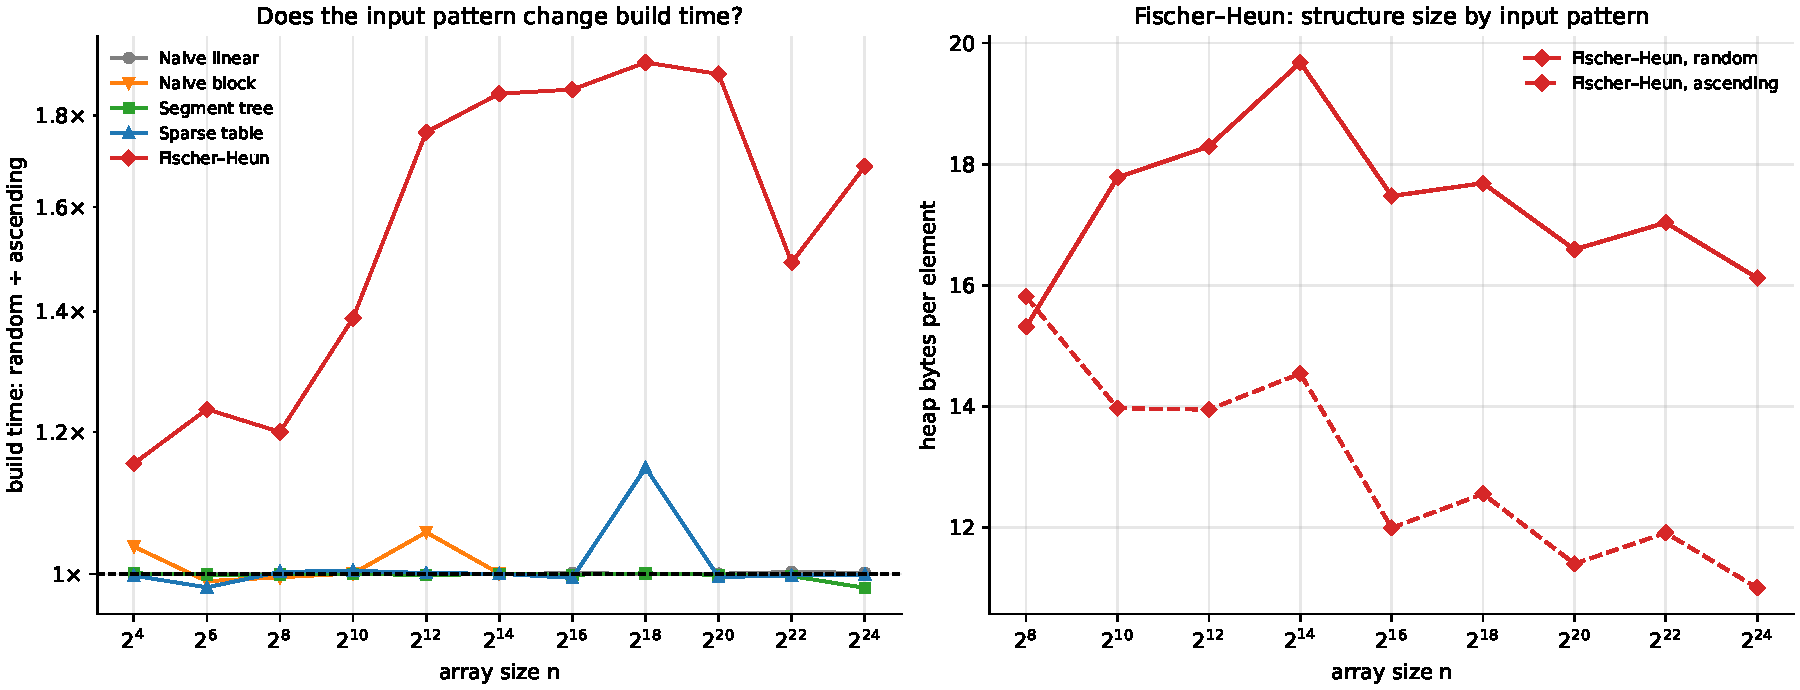
\includegraphics[width=0.8\linewidth]{figures/C1_pattern_sensitivity.pdf}
  \caption[Pattern sensitivity]{%
    Both randomised and ascending input arrays.  Can take up to 1.9 times longer depending on the number of unique blocks.}
  \label{fig:c1}
\end{figure}
Figure~\ref{fig:c1} shows that Fischer--Heun is the only structure consistently affected by input order, as its work depends on the block sizes of length $\frac{1}{2} \log_2 n$. During construction, each block's Cartesian number is checked in a hash map to see whether it has already been processed. In ascending input, every block has the same shape apart from a possible shorter final block, so it needs only one or two tables. Random input needs many tables, which makes its build up to 1.9 times slower and adds about 5 bytes per element. The spikes at $n = 2^{12}$ for Naive block and $n = 2^{18}$ for the sparse table are not input effects, as neither build depends on its values and both spikes changed with benchmark order. They are likely artefacts of allocator state left by earlier benchmarks, and do not affect the conclusion.


\begin{figure}[H]
  \centering
  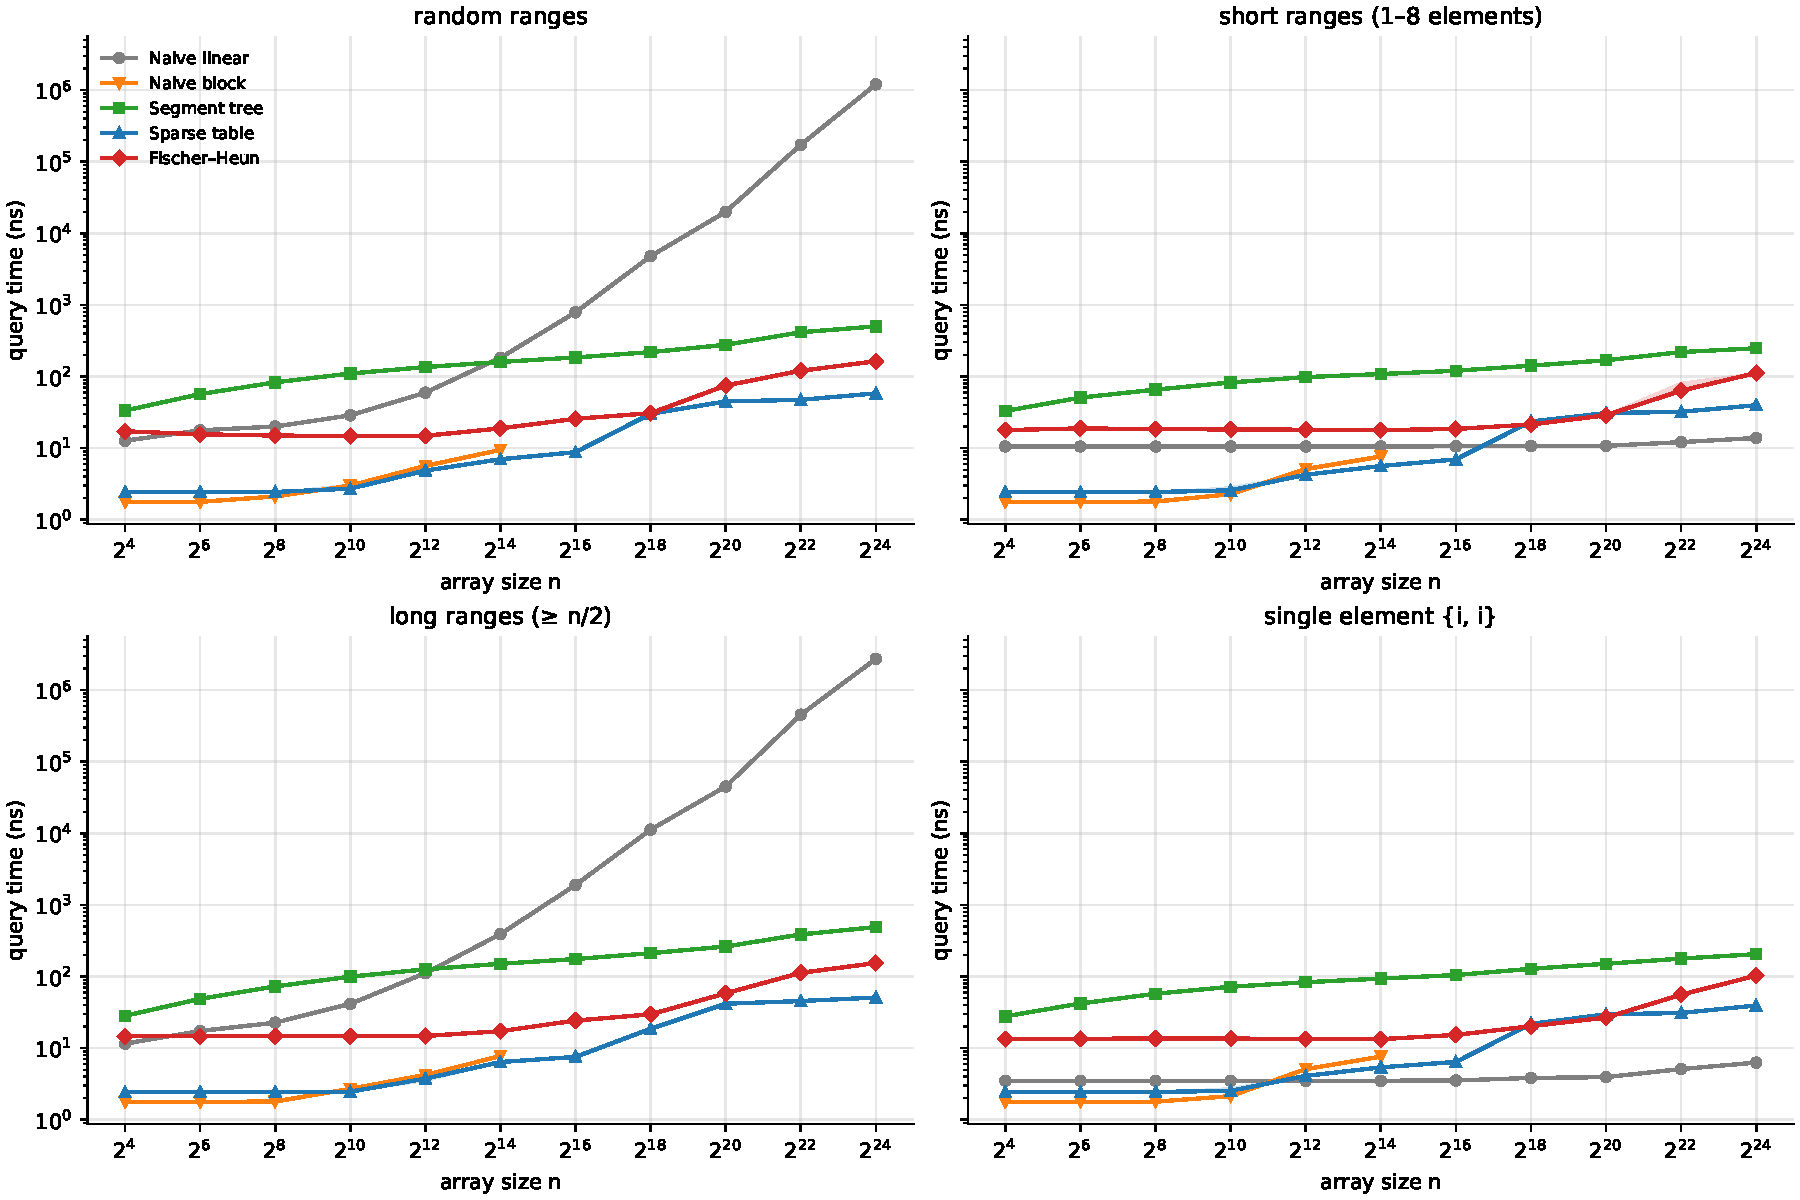
\includegraphics[width=0.8\linewidth]{figures/D1_query_time_by_pattern.pdf}
  \caption[Query by pattern time]{%
    Four possible query ranges checked: random, short, long, single.  Linear is the only largely affected.}
  \label{fig:d1}
\end{figure}
Figure~\ref{fig:d1} shows that the best structure for queries depends on range length. On random and long ranges, Naive block is fastest up to $n = 2^{8}$ and the sparse table from $n = 2^{10}$. On short and single-element ranges, Naive linear is fastest at large sizes, taking 13.9\,ns on short ranges at $n = 2^{24}$ against 39.7\,ns for the sparse table, as it only needs to read a few neighbouring values. Although the sparse table and Fischer--Heun perform a fixed number of steps per query, their random-range query times rise by factors of about 24 and 10 from $n = 2^{4}$ to $n = 2^{24}$. Asymptotic complexity alone therefore does not predict query time.

\begin{figure}[H]
  \centering
  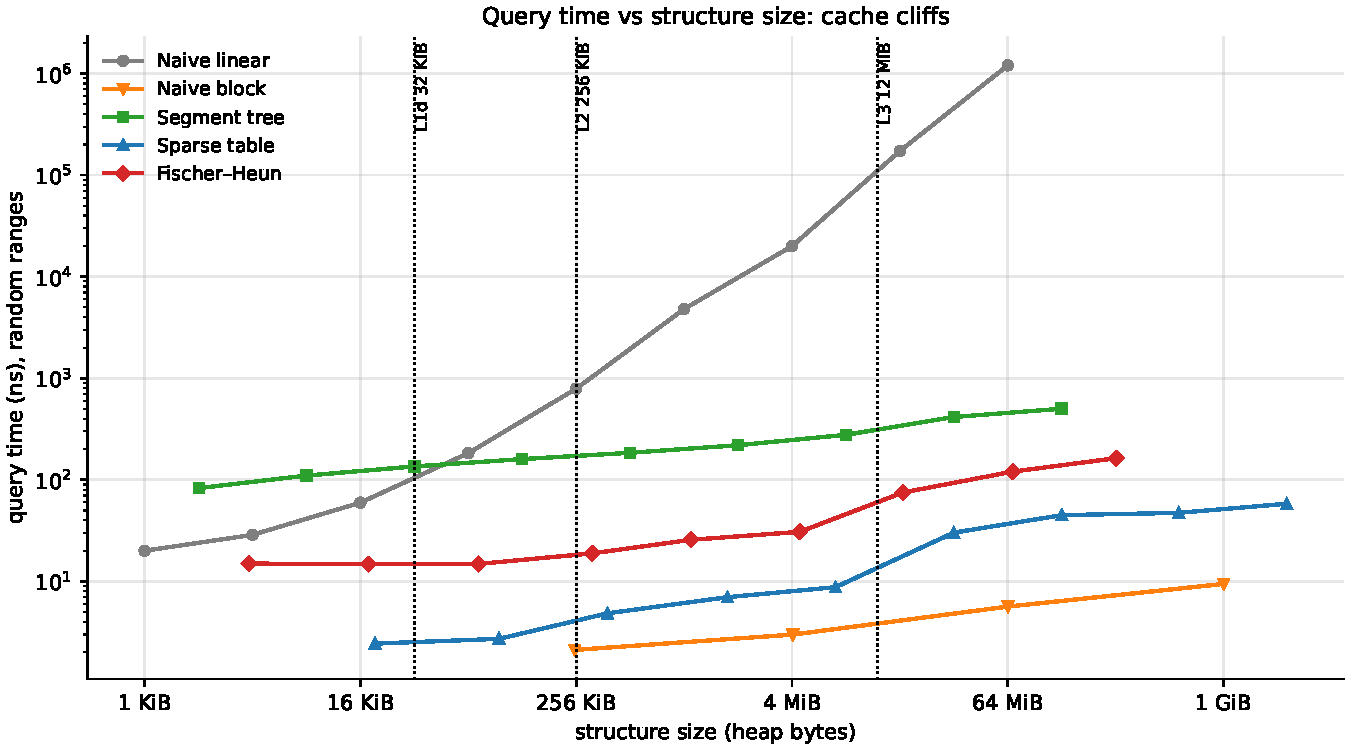
\includegraphics[width=0.8\linewidth]{figures/D2_cache_cliffs.pdf}
  \caption[Cache]{%
    Query time compared to structure size on heap.  Linear is the most affected, however all trend upwards after exceeding L3 cache size.}
  \label{fig:d2}
\end{figure}
Plotting query time against structure size in Figure~\ref{fig:d2} shows little change across the L1 and L2 boundaries, but a sharp rise beyond the 12\,MiB L3 cache. As they exceed it, the sparse table rises from 8.8\,ns to 30.2\,ns and Fischer--Heun from 30.8\,ns to 74.9\,ns, which is consistent with cache misses. The segment tree rises smoothly instead, which is consistent with its upper levels remaining cached. Increasing the query batch from $2^{16}$ to $2^{22}$ changed these results by less than 30\%, so the fixed batch does not explain this behaviour.

\begin{figure}[H]
  \centering
  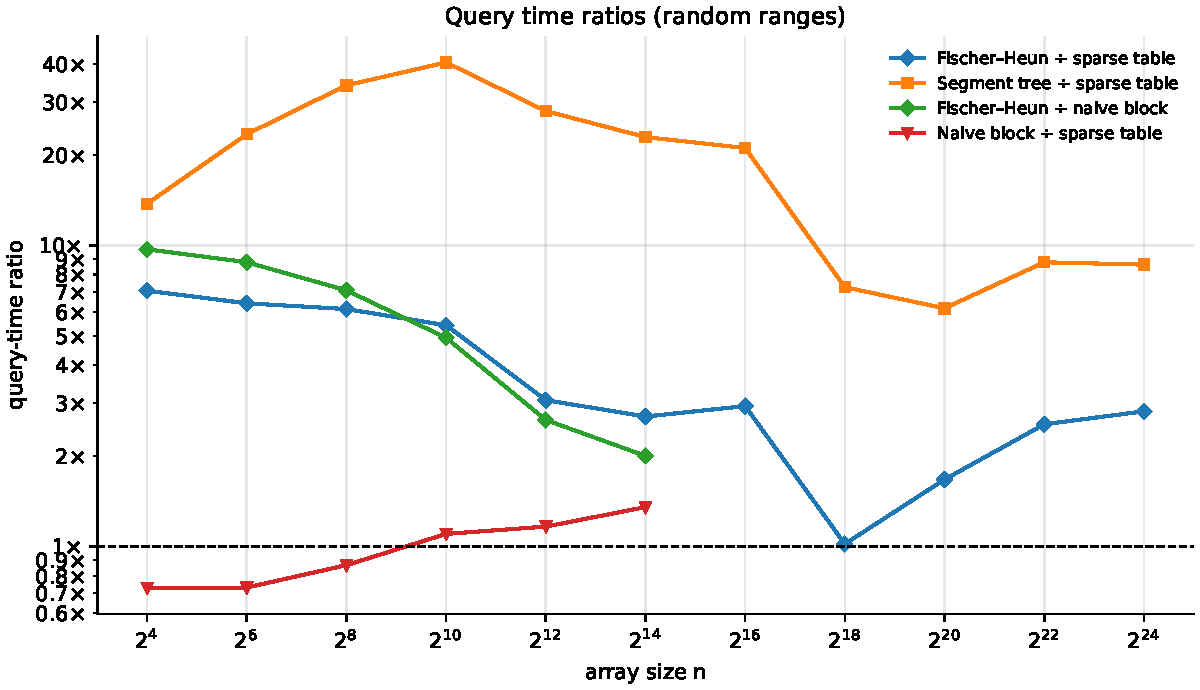
\includegraphics[width=0.8\linewidth]{figures/D3_query_ratios.pdf}
  \caption[Query ratios]{%
    Difference in query time for algorithms on randomised ranges.  Block and sparse are most similar, whilst segment tree and sparse table are most different.}
  \label{fig:d3}
\end{figure}
Figure~\ref{fig:d3} shows how the gaps between structures change with size. The segment tree is 14 to 41 times slower than the sparse table up to $n = 2^{16}$, then 6 to 9 times slower once the sparse table exceeds the L3 cache. Fischer--Heun's gap narrows from about 7 times at $n = 2^{4}$ to 1.02 at $n = 2^{18}$, where only the sparse table has exceeded L3, before widening to about 2.8 times at $n = 2^{24}$. Naive block starts about 27\% faster than the sparse table but becomes 35\% slower by $n = 2^{14}$, as its table grows quadratically.

\begin{figure}[H]
  \centering
  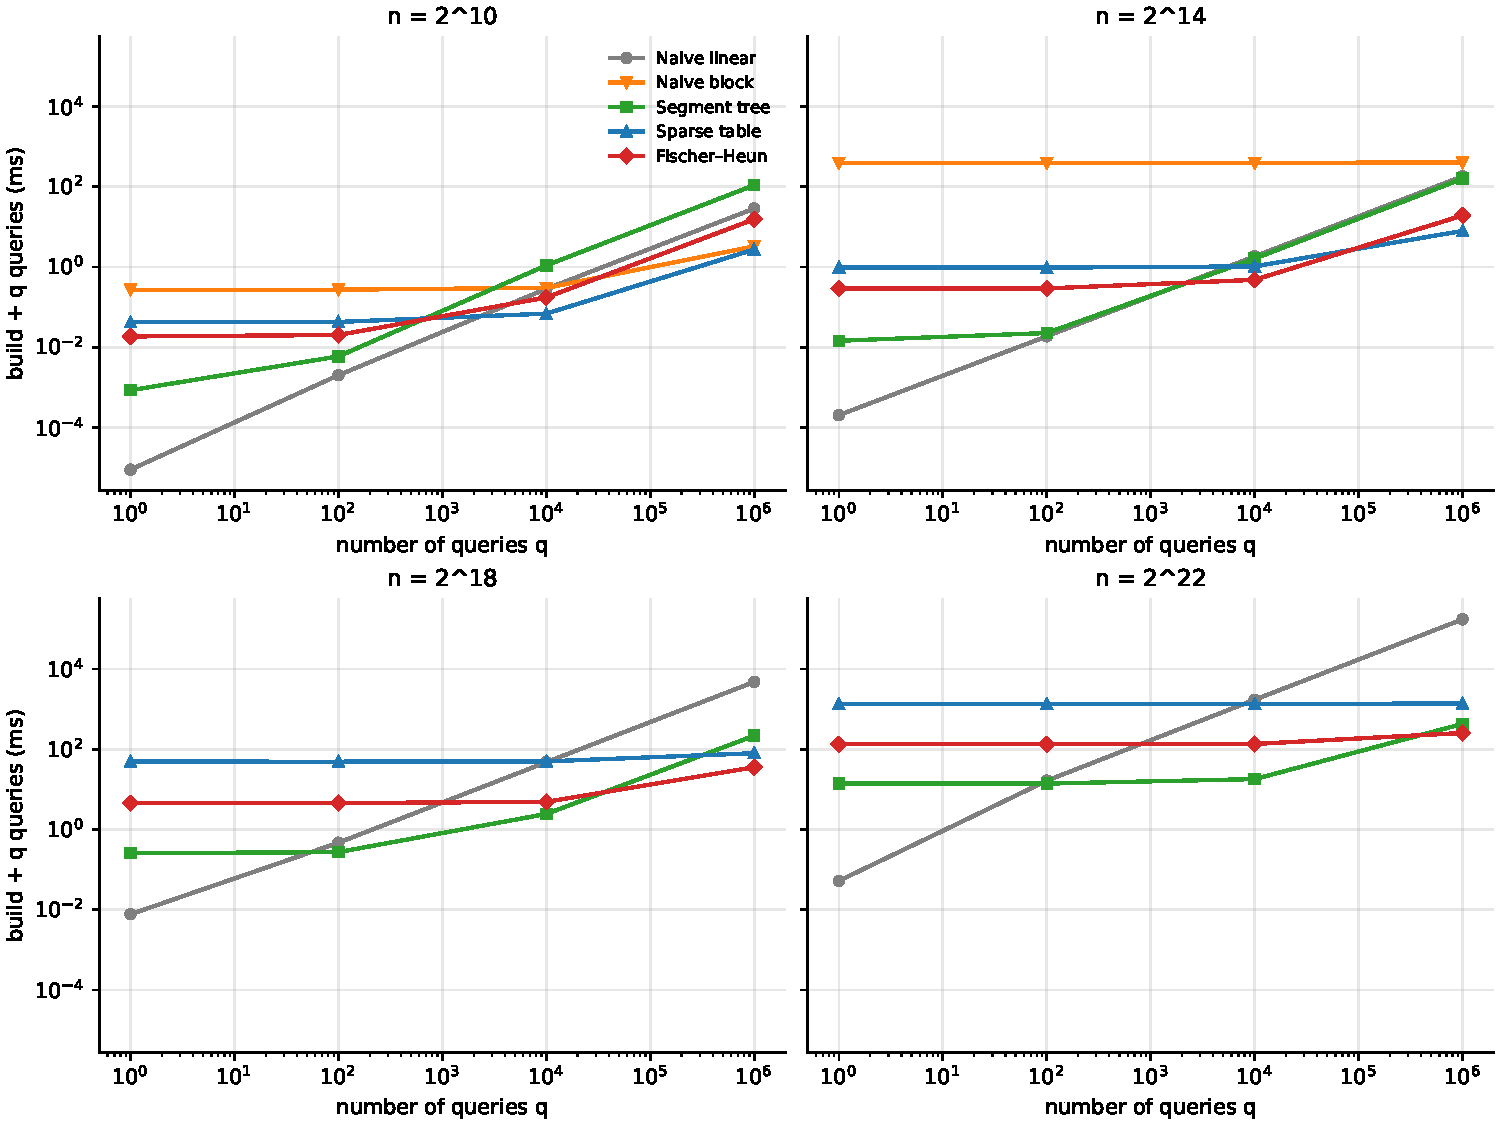
\includegraphics[width=\linewidth]{figures/E1_break_even.pdf}
  \caption[Break even]{%
    The slowest / fastest build time at array size n.  Ranges from $2^4$ to  $2^{24}$ with the exception of Linear.}
  \label{fig:e1}
\end{figure}
Figure~\ref{fig:e1} shows when an expensive build is worthwhile. At low query counts, build time dominates and each line stays flat, while Naive linear rises steadily as it has almost no build cost. At $n = 2^{22}$, the sparse table takes 1,346\,ms for one query and only 1,393\,ms for one million, because its build accounts for nearly all of the total. Over the same range, Naive linear rises from 0.05\,ms to about 175\,seconds. Queries cycle through a fixed batch of 65,536 ranges, so the largest query counts repeat earlier queries.

\begin{figure}[H]
  \centering
  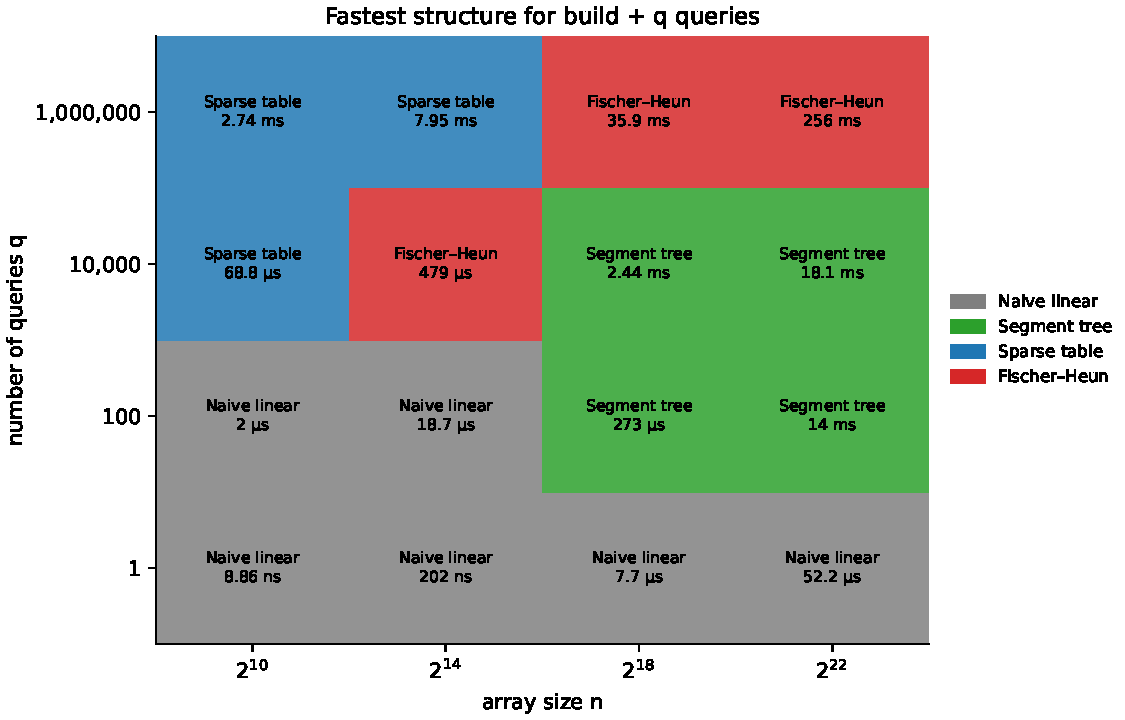
\includegraphics[width=0.8\linewidth]{figures/E2_winner_map.pdf}
  \caption[Fastest structure]{%
    Each cell is the algorithm with the lowest total median time for building, then answering q queries against four different sizes.  Linear dominates on smaller array or queries, whilst Fischer--Heun for large array with many queries.  Block wins nowhere.}
  \label{fig:e2}
\end{figure}
Figure~\ref{fig:e2} shows that no single structure is best for every workload. Naive linear is fastest for a single query at every size, and also for 100 queries up to $n = 2^{14}$. The segment tree wins moderate workloads on large arrays, taking 18.1\,ms for 10,000 queries at $n = 2^{22}$. Fischer--Heun wins one million queries from $n = 2^{18}$, taking 256\,ms at $n = 2^{22}$ against 430\,ms for the segment tree and 1,393\,ms for the sparse table. The sparse table wins only heavy workloads on smaller arrays, where its build cost can be repaid, and Naive block never wins.

\begin{figure}[H]
  \centering
  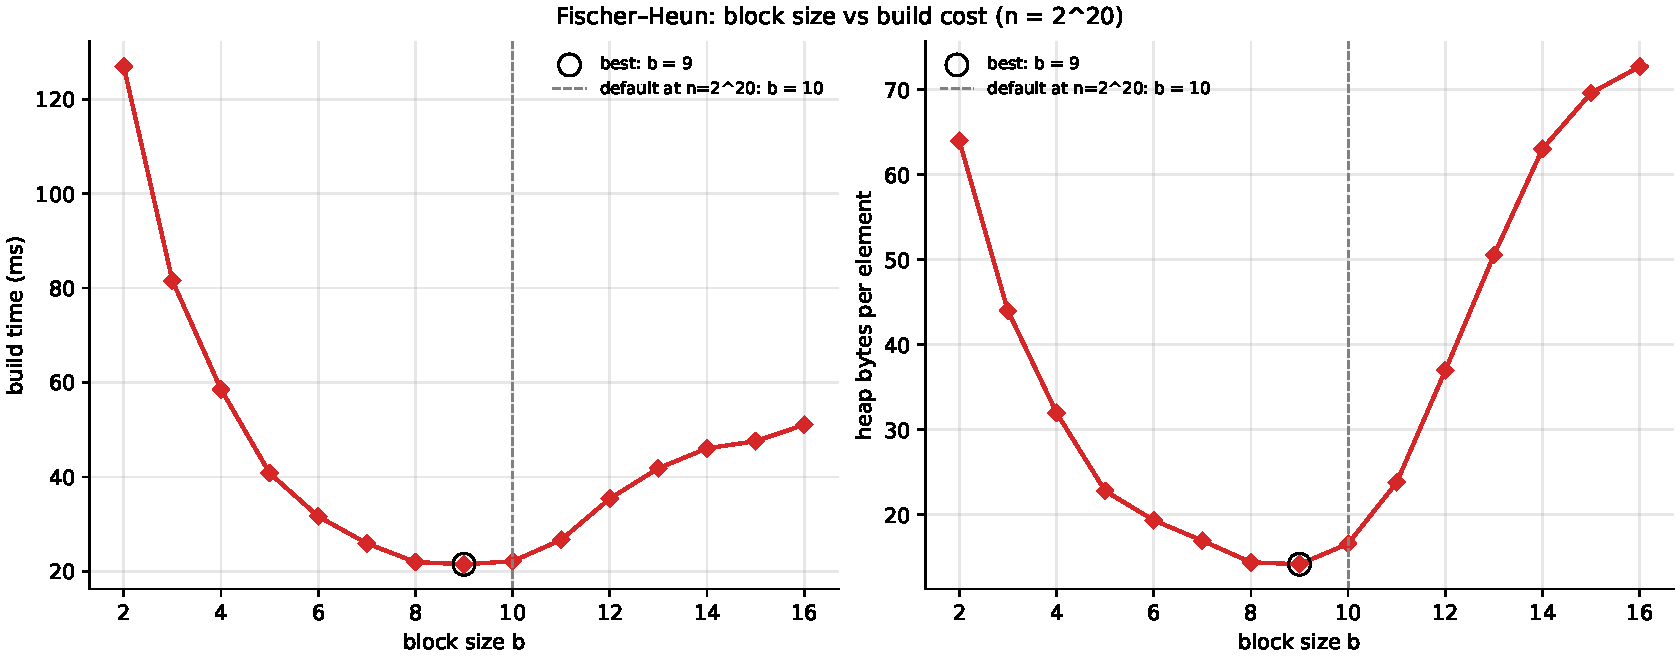
\includegraphics[width=0.8\linewidth]{figures/F1_fh_block_size.pdf}
  \caption[Fischer--Heun block size]{%
    Special case.  The affect of block size on total build time and memory consumption on heap.  The ideal is prove $\frac{1}{2}\cdot \log_2{n}$}.
  \label{fig:f1}
\end{figure}
Figure~\ref{fig:f1} shows a clear trade-off in Fischer--Heun's build at $n = 2^{20}$. Build time and memory are both lowest at $b = 9$, at 21.5\,ms and 14.2 bytes per element. Smaller blocks are costly because the sparse table covers more blocks, reaching 127\,ms and 64 bytes at $b = 2$. Larger blocks are costly because more distinct shapes each need a larger table, reaching 51\,ms and 73 bytes at $b = 16$. The default of $b = 10$ costs about 3\% more build time and 17\% more memory than $b = 9$, so the theoretical choice is close to optimal in practice. Query time was not measured at each block size, so this result covers build cost only.

\subsection{What Was Surprising}
There were several surprising things.  Firstly, the fact that the Fischer--Heun is a genuinely feasible implementation is interesting.  My initial thoughts were that it's an algorithm which chooses to associate n with everything in a way to lower complexity whilst being rather infeasible.  Secondly, the segment tree being the most optimal in many cases was interesting given I leaned towards the sparse table.  The idea of pre-computing ranges then taking the min of a combination sounded the most optimal, indeed I was incorrect.  Thirdly, the way the way memory is accessed by the algorithm and code.  Just because the block is pre-computed $n\times n$, doesn't mean it's an instant query for exceptionally large values.

\subsection{What We Would Do Next}
Firstly, I would like to spend a lot more time on this document giving it the treatment it deserves: an in-depth introduction and overview, worked examples, theoretical proofs for complexity and overall correctness, predictions which also consider growth-rates and computer hardware, benchmarking with different seeds and using different hardware in general; and lastly being able to formulate those proofs in something like Lean 4.  There is a lot to consider here, and the work was thoroughly enjoyable, however so much more can be done with these algorithms.

\section{Individual Contributions}
\subsection{Jay}
I have contributed through being the primary author of the sparse table, consisting of it's implementation, passing of all tests, following the group's error-handling conventions. I have also written the complexity analysis for the sparse table (Section 2.4) which covers the sparse table's description, correctness argument, running time and memory analysis. I have also recorded the sparse table breakdown/walkthrough segment.

\subsection{Nick}
I initialised the repository on GitHub, and then set up all the necessary building scripts, folders, include and src folders.  Within the Include, I created a common header file and all of the other header files for each implementation. I wrote all unit tests and their cases, all benchmarks, generators and helper functions.  The Fischer--Heun implementation was also completed by me, along with the linear and block.  I ran all of the benchmarks locally, wrote report sections introduction, analyses for linear, block and Fischer--Heun, comparisons, predictions, experimental methodology and every benchmarking analysis.  I then finished off the \textit{What surprised you} and \textit{What we'd do next} sections, as well as their video recordings. 

\subsection{James}
For this report, I have contributed by being the main author for the Segment Tree algorithm, creating the implementation, adapting to the common abstraction for all three implementations, and testing it against test cases that are created by Nick. Aside from the primary algorithm, I have discussed a few points from our list of predictions, stating whether it could be a “good” prediction, an outcome that we’re uncertain about, or it would be a “bad” prediction, ones that easily disproven before the analysis could even begin. I have also taken the raw data, using Nick’s computer as the local benchmark, and created graph visualisations to test against our predictions in this research. Lastly, I have taken the lead in initialising the video process, delegating roles to my groupmate where it is most convenient to everyone under life circumstances.
\section{Reflections}
\subsection{Jay}
The sparse table has no worst-case input pattern. Construction always does the same work for a given $n$, as every power $p$ fills $n - 2^{p} + 1$ entries regardless of the values. A query is always two table reads and one comparison, so sorted, reversed, random and all-equal arrays of the same length cost the same. The real worst case comes from the size of the input. Memory grows as $n(\lfloor \log_2 n \rfloor + 1)$ integers, which is roughly 84\,MiB at $n = 2^{20}$, compared to 4\,MiB for the array itself. The other bad case is a large array with very few queries. The $\Theta(n \log n)$ build is then paid up front and never recovered, while the segment tree builds in $O(n)$.
\\
\\
A design decision I faced was the table layout. The initial version of the implementation was aided by AI, and stored the table as \texttt{table[k][i]}, with one row per power. I later switched to \texttt{sparseTable[i][power]}, with one row per start index, to match the sparse table inside Fischer--Heun. Both layouts give identical answers, but matching them means our benchmarks compare the algorithms rather than two different memory layouts. I also had issues configuring Google Benchmark's regex check, as the MinGW runtime DLLs were not on \texttt{PATH}. Adding the compiler's \texttt{bin} folder to \texttt{PATH} and deleting the cache resolved this issue.
\\
\\
Every row is allocated at full width, even though column $p$ only uses $n - 2^{p} + 1$ entries. Each row is also a separate vector, so the table makes $n$ separate allocations. I would size each column to what it uses, or store the whole table in one flat array indexed as \texttt{power * n + i}.
\\
\\
Initially, I did not understand why a query could use two blocks that overlap. Choosing $p = \lfloor \log_2 m \rfloor$ for a range of length $m$ gives $2^{p} \le m < 2^{p+1}$. Each block is no longer than the range, so it stays inside it. Together, the two blocks are at least as long as the range, so they cover it completely. The overlapping elements are counted twice, which does not matter since $\min(v, v) = v$. This is also why the structure only works for idempotent operations such as $\min$.

\subsection{Nick}
AI was particularly useful for explaining the precise implementation of my peers.  Whilst I knew the algorithms and how they operated, there can be tweaks and caveats which AI can explain far easier.  The best example of this was the first time reading sparse table, I had mistaken it for running $O(n^2)$, when AI picked up me misreading the for loop statement (a very simple yet dangerous mistake).  There was no situation where group work was threatened.

\subsection{James}
When it comes to the worst case that may occur in the Segment Tree, in terms of time, would depend entirely on the query range, not the data itself, since the build is $\Theta(n)$ and query is $\Theta(\log n)$. When it comes to memory allocation, the worst case is n=2k+1 since the tree pads 2k+1 leaves, so it needs about 4n ints. Looking through the benchmark, measuring 12 bytes/element versus 8 at n = 2k, the build time nearly doubled, although it would not be considered the worst case because if the query range is also large in this build of the segment tree, it could trigger a long search throughout the tree, making the time it takes longer.
\\
\\
When I first designed the variable “leaves” in the implementation file, I was fairly new at working with a local segmentTree which holds the member variables for the implementation. The implementation failed multiple times, and it took multiple attempts to realise that initialising the variable within the implementation (e.g leaves {1}) completely overwrites the member variables, which does not allow the leaves member to be accessed properly during the building of the tree.
\\
\\
Another thing during the implementation, Nick had given me a scaffold of the implementation tree, a ghost of a Query function. Since I believe that Query function should be a simple function that calls a helper function, which can help with modularity, I decided to design rangeMin function that can pass all essential parameters to complete the query properly, allowing the actual Query function to just call the helper function for easier readability in the code.
\\
\\
If I could’ve done something differently in this assignment, I wish I could have helped Nick designed more of the fundamental level of the code, ensuring that the query was inclusive from left to right in the first face, and learned beforehand that MSVC is not always compatible with other IDE/work environment (e.g compared to builds that were done on MAC or Linux. MSVC did not understand -Wextra, it would only understand /W4).
\\
\\
A few things I didn’t fully understand before working on this report is being oblivious to how MSVC interacts with the CMake build, which prompted me to look further into the matter (as noted above). Another thing was that during the implementation, I did not fully grasp how binary trees are built on an array, and how a parent node would start accessing its children node (via 2i+1, 2i+2, that math was confusing at the time). And lastly, I was completely new to using Overleaf for writing the report with my groupmate, so it took a few hours for me to grasp the basic understanding of how to format in the actual report itself.
\section{Use of AI}
\subsection{Jay}
AI was utilised throughout my contributions to the project (specifically Claude). It was initially used as one of my methods of conceptual understanding of sparse tables, to which it assisted me in my draft implementation of the algorithm, which was later reworked and polished (e.g. naming convention changes and comments to be more aligned with my groupmates code). It was also used for the structuring the draft of my reflection. I also had used it to create my visualisation slide of the sparse table in the implementations walkthrough, and as a general guideline of how I should go about presenting my algorithm.
\\
\\
Claude suggested to follow exclusive [a, b) ranges initially, which wasn't useful as our groups shared test use inclusive ranges instead, (e.g. {4, 4} as a valid single-element query).
Coding against this would have put every query off by one, so the final implementation followed the tests in tests/common.h, which were used as the correct approach instead.
\\
\\
Through my usage of Claude in a groupwork environment, I had found it to be more tedious at certain points opposed to convenient, through working with others, questions I had regarding the assignment would of required me to paste in group chat messages or shared tests to provide Claude with enough context to assist me in giving me a useful answer. Along with this, through my assigned work, I also had minimal incentive to understand groupmates algorithms beyond a very high level, without AI use I'd assume I'd have needed to engaged more directly with their code.
\subsection{Nick}
\subsubsection{Tool Use}
The only AI models used were \textit{Claude Opus 5.5 and 5.1 Medium (05/11/2026)}. My entire implementation of Fischer--Heun was hand-written, without any AI assistance.  When writing tests, I used AI to generate me most of the actual cases, including edge cases because I didn't want to write them all by hand.  Then for benchmarking I heavily relied on back and forth querying with the AI, on how to construct my benchmarks, but they were all written by myself as I wanted to learn the library.
\\
\\
For the report, AI was heavily used to correct all my wording and reasoning (I initially write then Claude fixes the errors and makes it nice).  For the theoretical analysis, I wrote the initial, and then had AI check and fix any notation mistakes.  Then, I also used it to write the pseudocode under my exact querying.  For the analyses, I would pass the chart through AI to see if it would pick up on anything I could've missed for an overall better analysis.  There was also assistance with referencing materials I gathered.
\subsubsection{Incorrections}
One notable trouble I had with Claude was analysing the strange segment tree drop at $n = 2^{22}$ in Figure~\ref{fig:a3}.  Claude believed it was the exact point which the segment tree surpassed L3 cache limit, and therefore it became slower whilst Fischer--Heun remained the same.  I insisted to Claude there is no way a jump that large could be caused by leaving the cache, and that sharply.  Then it checked again, and it turns out the issue was the fact that $2^{22}$ is exactly the limit of glibc allocating memory.  So a similar affect to leaving L3, such that each next array must call the operating system.
\\
\\
Another was that I asked for the cause of Figure~\ref{fig:a2} naive block jumping at $n = 2^{10}$.  The response was that it lines up with L3, and therefore the cause of taking longer to build is asking the operating system for more memory.  At the time, I was not entirely familiar with L3 so I interrogated and asked what it was.  This allowed me to learn more about the use of CPU caches, however in the process of explaining Claude decided to rerun benchmarks.  It concluded that the jump was too large for L3, despite the timing being right.  The actual problem is that every time past L3 memory is freed, the program can't just cache it, instead it needs to re-call the operating system, taking far longer.  I find this my most interesting use as I didn't even know the answer, yet it corrected itself after further analysis.
\\
\\
Lastly, when getting AI to assist with writing benchmarks, we concluded that ranging all the way from $2^4$ to $2^{24}$ would be enough.  Then once complete I would run, and it took incredibly long, was slow and even crashed.  The actual reason was that Claude convinced me to check block up to that range, which would be $2^{48}$, requiring roughly a single petabyte of memory.  I only figured the calculation out after doing some tweaking with what values worked.  This was an easy to catch example because the benchmarks need to all run locally and I need to moderate, however it's easy to see how this could cause bugs if it were deep inside an implementation.

\subsection{James}
My AI use when implementing the Segment Tree algorithm was minimal, as I use Claude to help check on any syntax errors and check against test cases (due to my IDE being primarily on Visual Studio). The rest of my implementation is based on Roy's explanation ~\cite{roy2015}.  I also have used Claude heavily in implementing the python notebook for plotting graphs and values for the analysis section, checking against the list of predictions my groupmate has made for the report. Lastly, I have used ChatGPT mildly when working on the video, using it to assist in writing a general script for my introduction section, but then I went on my bullet point notes to assist on my Segment Tree algorithm section.
\\
\\
During my conversation with Claude in checking the list of potential predictions we could use for testing, Claude flagged that “Naive Block consumes the most memory for larger values” as obsolete, as Naive Block grows in O(n)2. I noted this concern to Nick, to which he reasoned that we wouldn’t know for sure, as under very certain circumstances that an algorithm like Fischer--Heun might be worse than Block, raising the fact that Fischer--Heun is as fast as Linear where log2(a) < 2. In the end, since we’re observing at what point is each algorithm the best, we have decided to write off this claim to have the prediction checked during analysis.
\\
\\
Besides all of this AI, my utilisation of AI in this group work had helped me significantly in catching up to speed on both Sparse Tree and Fischer--Heun algorithm, allowing me to understand it a little deeper than the surface level and raise questions during comparison of the three implementations. I believe that learning how to use AI in this way will be of great benefit to the person’s knowledge and experience, instead of researching from multiple sources at once.

\section{References}
\begin{thebibliography}{99}
\bibitem{fischer2006} J. Fischer and V. Heun, ``Theoretical and practical improvements on the RMQ-problem, with applications to LCA and LCE,'' in \emph{Proc. Combinatorial Pattern Matching}, vol. 4009, Springer, 2006, pp. 36--48.

\bibitem{bender2000} M. A. Bender and M. Farach-Colton, ``The LCA problem revisited,'' in \emph{Proc. LATIN 2000: Theoretical Informatics}, vol. 1776, Springer, 2000, pp. 88--94.

\bibitem{cs166rmq1} K. Schwarz, ``Range minimum queries, part one,'' lecture slides, CS166: Data Structures, Stanford Univ., Stanford, CA, USA, Spring 2021. Accessed: Nov. 5, 2026. [Online]. Available: \url{https://web.stanford.edu/class/archive/cs/cs166/cs166.1216/lectures/00/Slides00.pdf}

\bibitem{cs166rmq2} K. Schwarz, ``Range minimum queries, part two,'' lecture slides, CS166: Data Structures, Stanford Univ., Stanford, CA, USA, Spring 2021. Accessed: Nov. 5, 2026. [Online]. Available: \url{https://web.stanford.edu/class/archive/cs/cs166/cs166.1216/lectures/01/Slides01.pdf}

\bibitem{mit6851static} MIT OpenCourseWare, \emph{15. Static Trees}. (2012). Accessed: Nov. 5, 2026. [Online Video]. Available: \url{https://www.youtube.com/watch?v=0rCFkuQS968}

\bibitem{roy2015} T. Roy, \emph{Segment Tree Range Minimum Query}. (Apr. 22, 2015). Accessed: Nov. 6, 2026. [Online Video]. Available: \url{https://www.youtube.com/watch?v=ZBHKZF5w4YU}

\end{thebibliography}
\end{document}
